\documentclass[tikz,border=10pt]{standalone}
\usetikzlibrary{calc}
\begin{document}
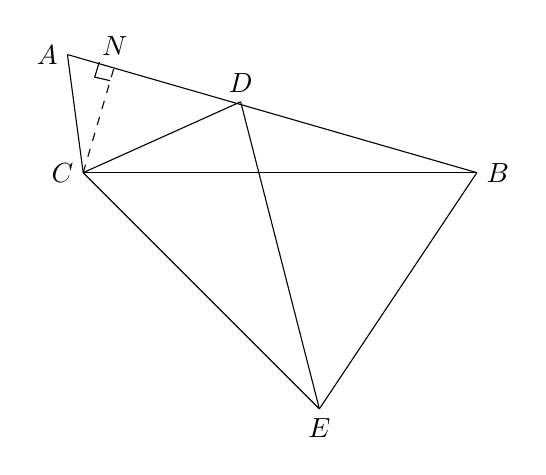
\begin{tikzpicture}
    \coordinate (C) at (0, 0);
    \coordinate (B) at (5, 0);
    \coordinate (A) at (-0.2, 1.5);
    \coordinate (D) at (2, 0.9);
    \coordinate (N) at (0.4, 1.36);
    \coordinate (E) at (3, -3);

    % Draw solid lines
    \draw (A) -- (B);
    \draw (A) -- (C);
    \draw (C) -- (B);
    \draw (C) -- (D);
    \draw (C) -- (E);
    \draw (B) -- (E);
    \draw (D) -- (E);

    % Draw dashed line
    \draw[dashed] (C) -- (N);

    % Right angle mark at N
    % Vector NC is roughly (-0.4, -1.36). Angle ~ 253 deg.
    % Vector NA is roughly (-0.6, 0.14). Angle ~ 167 deg.
    % Draw small square corner
    \coordinate (N1) at ($(N) + (253:0.2)$);
    \coordinate (N2) at ($(N) + (167:0.2)$);
    \draw (N1) -- ($(N1) + (N2) - (N)$) -- (N2);

    % Labels
    \node[left] at (A) {$A$};
    \node[above] at (N) {$N$};
    \node[above] at (D) {$D$};
    \node[left] at (C) {$C$};
    \node[right] at (B) {$B$};
    \node[below] at (E) {$E$};
\end{tikzpicture}
\end{document}
